\subsubsection{UC5 - Login con private key}
\begin{figure}[h]
	\centering
	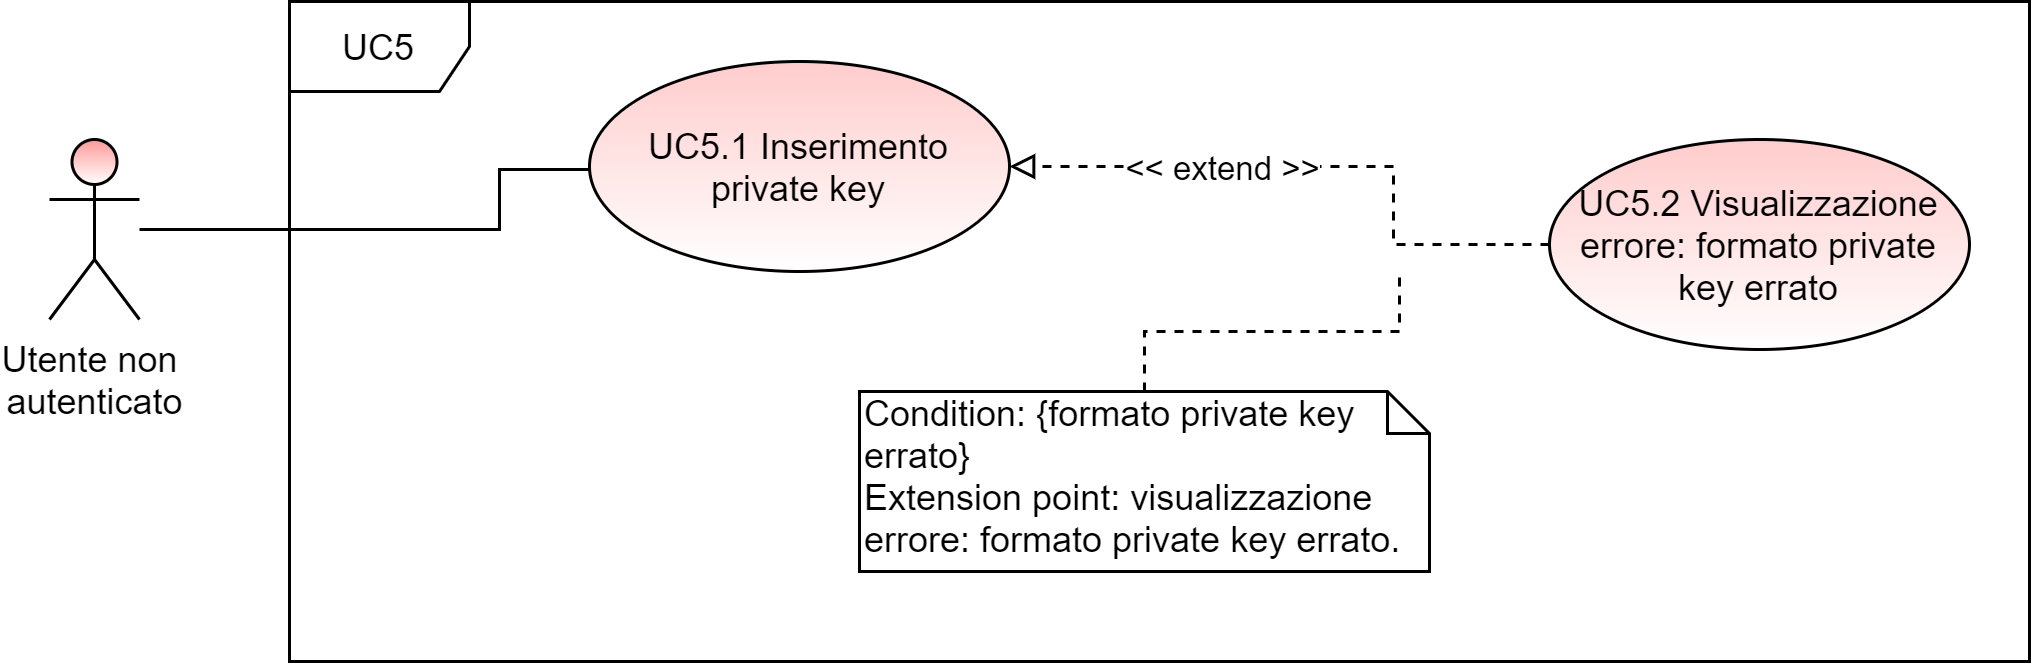
\includegraphics[scale=\ucs]{./res/img/UC5.png}
	\caption {UC5 - Login con private key}
\end{figure}
\begin{itemize}
	\item \textbf{Attori primari:} \una{};
	\item \textbf{Attori secondari:} \re{};
	\item \textbf{Descrizione:} l’utente può utilizzare il comando \ploginPrivate{} per autenticarsi all’interno della rete Ethereum\ped{\textit{G}}; 
	\item \textbf{Scenario principale:} l'utente esegue il comando \login{} indicando manualmente le credenziali necessarie; 
	\item \textbf{Precondizione:} l’utente tenta di autenticarsi alla piattaforma;
	\item \textbf{Postcondizione:} l’utente si è autenticato correttamente.
\end{itemize}
